\documentclass{beamer}

\usetheme{CambridgeUS}
\setbeamertemplate{footline}[frame number] % Affiche uniquement le numéro de page

% \setbeameroption{show notes on second screen=right} % Affiche les notes à droite
\usepackage[utf8]{inputenc}
\usepackage{graphicx}
\usepackage{hyperref}
\usepackage[T1]{fontenc}
\usepackage{caption}
\usepackage{placeins} % Required for \Floatbarrier

\title{Edge Computing: A Decentralized Evolution of the Cloud}
\author{Galiléa LE MOULLEC (Mun ID: 202415993) \and Félicien MOQUET (Mun ID: 202415994)}
\institute{Memorial University of Newfoundland, St. John's, Canada}
\date{March 2025}

\begin{document}

\begin{frame}
  \titlepage
\end{frame}

%--- Slide 1: Introduction ---
\begin{frame}{Introduction}
    \begin{block}{\textbf{Definition}}
    Edge computing is a
    distributed computing paradigm that integrates networking, computing, stor-
    age, and application resources \textbf{near data sources} to provide intelligent services
    with minimal delay. By processing and storing data closer to its origin, edge
    computing \textbf{minimizes latency}, \textbf{optimizes bandwidth usage}, and \textbf{enhances system
    responsiveness}
      \end{block}

\end{frame}

%--- Slide 2: Why Edge Computing? ---
\begin{frame}{Why Edge Computing?}
  \begin{itemize}
    \item \textbf{Latency:} Reduces delay for real-time responses
    \item \textbf{Bandwidth:} Minimizes data transfer volume
    \item \textbf{Privacy:} Keeps sensitive data local
    \item \textbf{Resilience:} Operates even with cloud disconnections
  \end{itemize}
  \note{
    In this video, we'll explore Edge Computing and its importance. Consider a startup that initially relies on cloud computing to manage financial data. As the company grows, real-time decisions are needed, making cloud computing inefficient. Instead, they hire an in-house accountant to process data locally, improving speed and decision-making.

    Edge Computing works similarly, by processing data closer to the source rather than relying on the cloud. Key benefits include:

    - **Latency:** Processing data locally reduces delays, which is vital for applications like smart cars or real-time sensors.
    - **Privacy:** Keeping sensitive data local minimizes the risk of exposure, especially in industries like healthcare.
    - **Bandwidth:** Instead of transmitting all data to the cloud, only relevant information is sent, reducing the need for high bandwidth.
    - **Resilience:** Edge devices continue to function even without cloud connectivity, ensuring uninterrupted service in critical situations.

    These benefits make Edge Computing essential for fast, private, and reliable applications, even when cloud services are unavailable.
  }
\end{frame}


%--- Slide 3: Architecture Overview ---
\begin{frame}{Architecture Overview}
  \begin{itemize}
    \item \textbf{Edge devices:} Sensors, wearables, cameras
    \item \textbf{Edge nodes:} Gateways, micro-servers, local processors
    \item \textbf{Cloud layer:} For large-scale analytics and storage
  \end{itemize}
  \vspace{0.5cm}
  \centering
  \begin{figure}
    \centering
    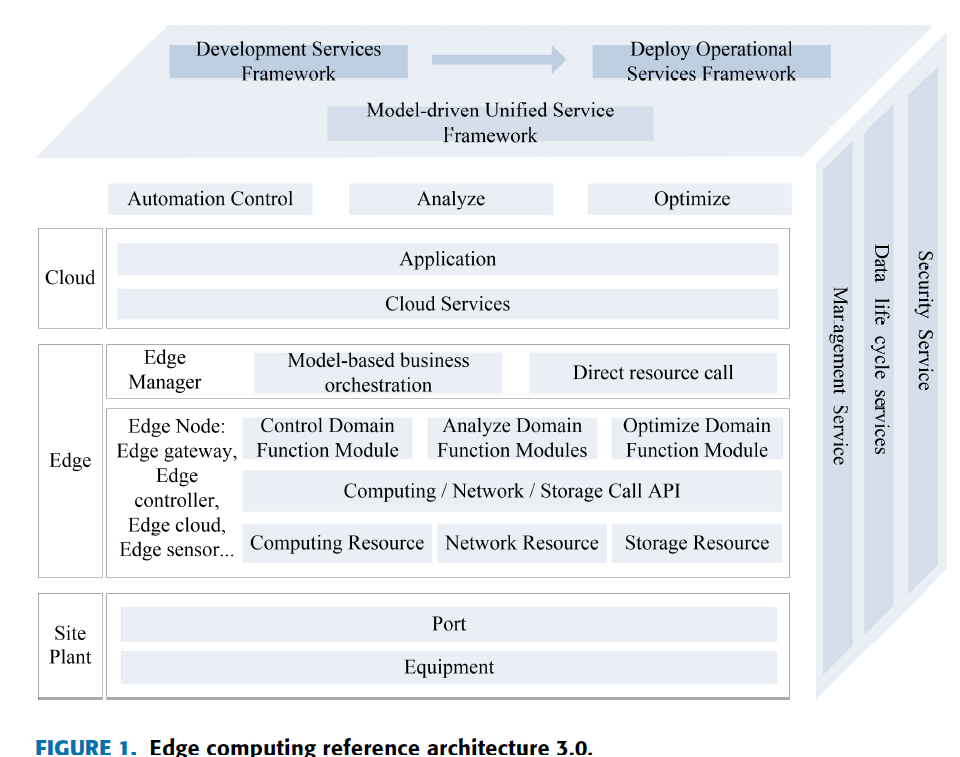
\includegraphics[width=0.5\linewidth]{IMG/6.png} % Optional
  \end{figure}
  \vspace{0.2cm}
  \small \textit{Figure 1: Edge computing reference architecture}
\end{frame}

%--- Slide 4: Use Case - IoT ---
\begin{frame}{Use Case: Internet of Things (IoT)}
  \begin{itemize}
    \item Smart homes: temperature, lighting, security
    \item Environmental monitoring: air quality, agriculture
    \item Local processing improves responsiveness and privacy
  \end{itemize}
  \vspace{0.5cm}
  \centering
  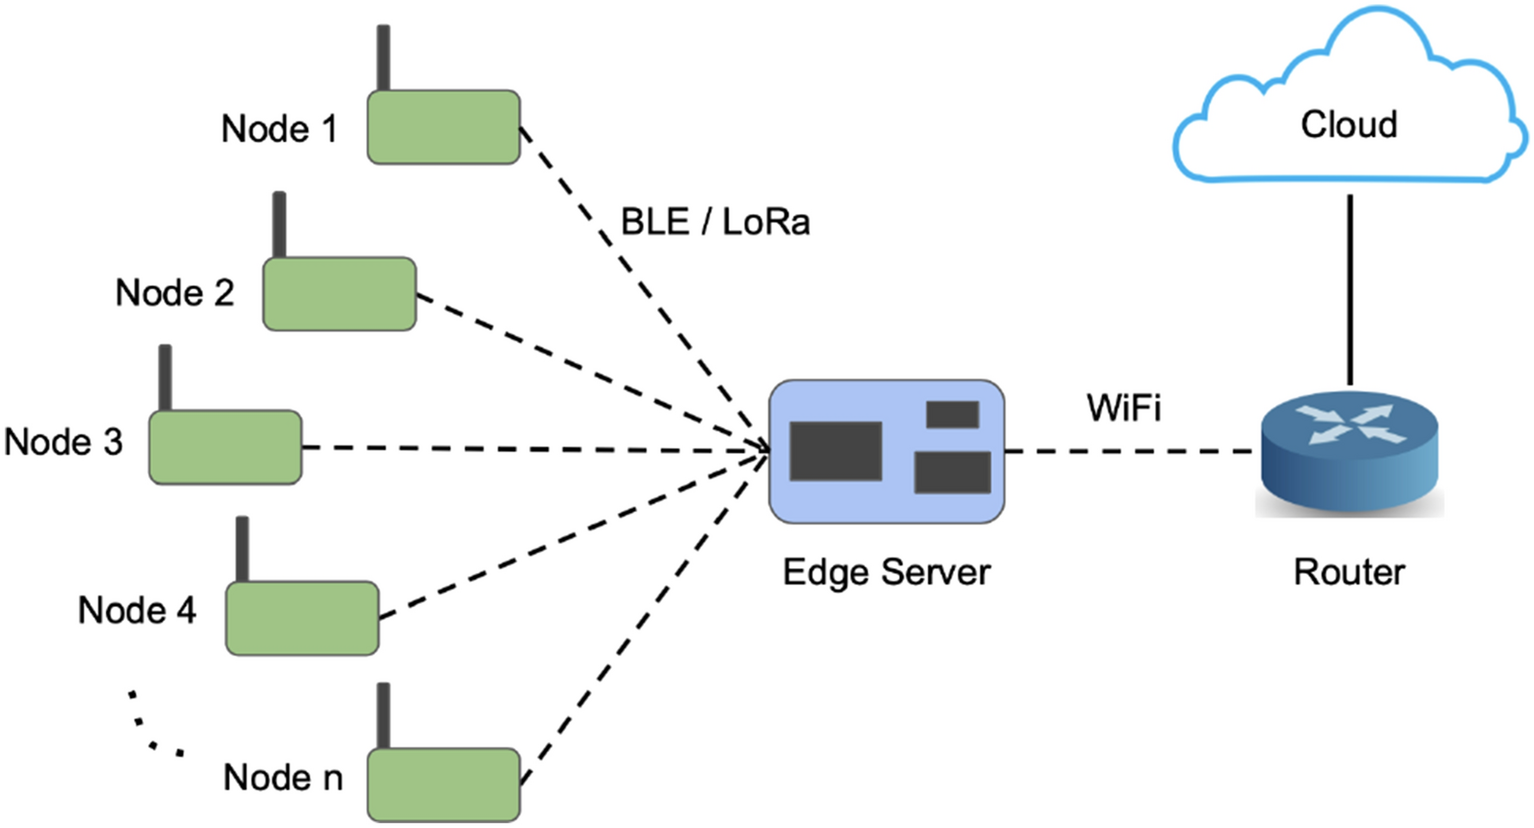
\includegraphics[width=0.6\linewidth]{IMG/12.png} % Optional
  \vspace{0.2cm}
  \small \textit{Figure 2: IoT use case}
  \note{
    IoT applications benefit from edge computing through fast reactions and privacy. In smart homes, sensors react immediately. In agriculture, edge devices adapt irrigation in real time.
  }
\end{frame}

%--- Slide 5: Use Case - Autonomous Vehicles ---
\begin{frame}{Use Case: Autonomous Vehicles}
  \begin{itemize}
    \item Onboard sensors generate huge data streams
    \item Requires instant decision-making (e.g. braking)
    \item Edge computing enables safety-critical operations
  \end{itemize}
  \vspace{0.2cm}
  \centering
  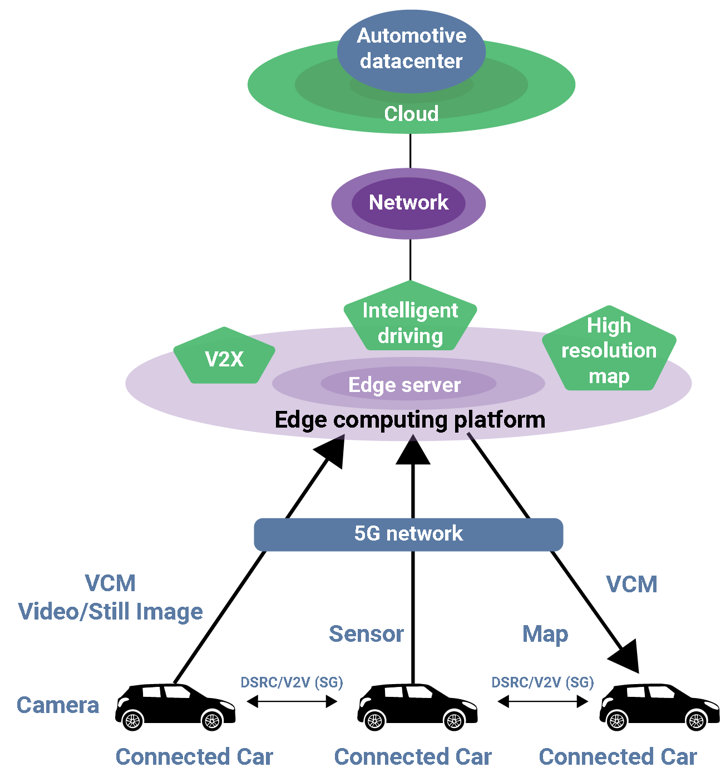
\includegraphics[width=0.4\linewidth]{IMG/13.png} % Optional
  \vspace{0.2cm}
  \small \textit{Figure 3: Autonomous vehicles use case}
\end{frame}

\begin{frame}{Use Case: Smart Cities}
    \begin{columns}[t]  % [t] pour aligner en haut
      % Colonne gauche : texte
      \begin{column}{0.5\textwidth}
        \begin{itemize}
          \item Real-time traffic management
          \item Public safety and surveillance
          \item Energy optimization and environmental monitoring
        \end{itemize}
      \end{column}
  
      % Colonne droite : image
      \begin{column}{0.5\textwidth}
        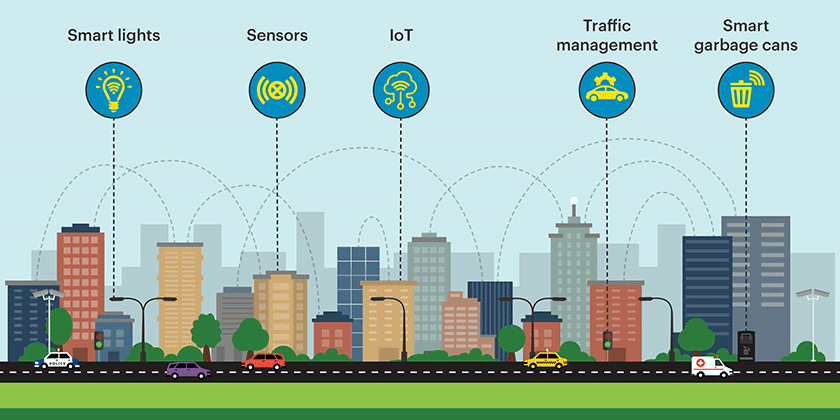
\includegraphics[width=\linewidth]{IMG/14.png}
        \vspace{0.2cm}
  
        \small \textit{Figure 4: Smart cities use case}
      \end{column}
    \end{columns}
  
    \note{
      Edge computing enables cities to be smarter and more efficient. Local processing in traffic lights and surveillance systems improves responsiveness and reduces network dependency.
    }
  \end{frame}
  

%--- Slide 7: Use Case - Healthcare ---
\begin{frame}{Use Case: Healthcare and Telemedicine}
  \begin{itemize}
    \item Real-time patient monitoring
    \item On-site diagnostics in emergencies
    \item Strong data privacy and compliance (e.g. GDPR)
  \end{itemize}
  \vspace{0.5cm}
  \centering
  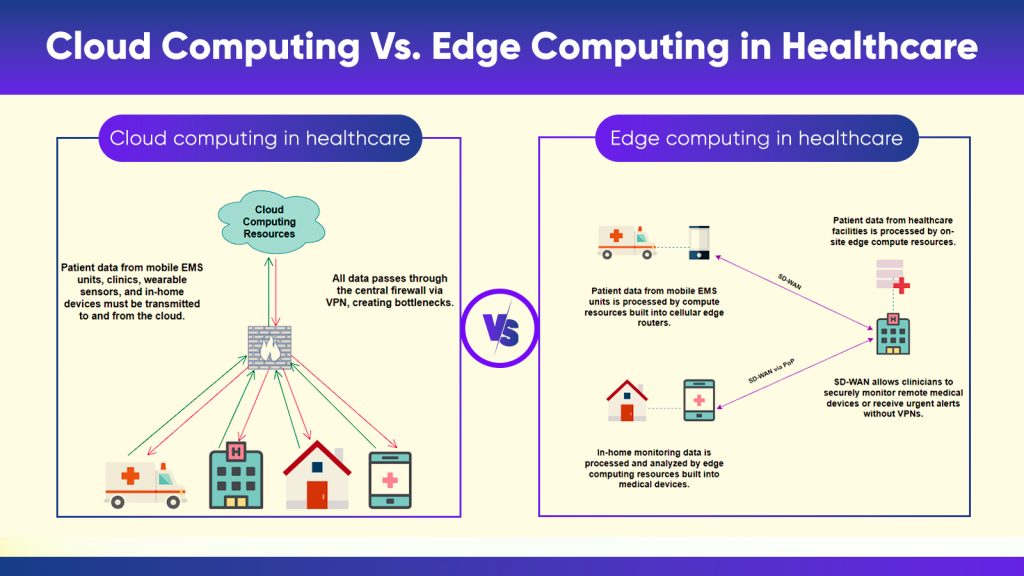
\includegraphics[width=0.6\linewidth]{IMG/15.jpg} % Optional
  \vspace{0.2cm}
  \small \textit{Figure 5: Healthcare use case}
\end{frame}

%--- Slide 8: Pros and Cons ---
\begin{frame}{Advantages and Challenges}
  \textbf{Advantages:}
  \begin{itemize}
    \item Lower latency and bandwidth usage
    \item Better data privacy and security
    \item Improved resilience and scalability
  \end{itemize}
  \vspace{0.3cm}
  \textbf{Challenges:}
  \begin{itemize}
    \item Complex management of distributed nodes
    \item Interoperability with cloud platforms
    \item Security at the edge
  \end{itemize}
  \note{
    While edge computing has many strengths, it introduces new challenges. Managing and securing distributed nodes is complex, and integration with existing cloud systems remains tricky.
  }
\end{frame}

%--- Slide 9: Trends and Future Perspectives ---
\begin{frame}{Trends and Future Perspectives}
  \begin{itemize}
    \item Integration with AI and 5G for smarter edge decisions
    \item Lightweight containers and orchestration (e.g. K3s)
    \item Research in privacy-preserving analytics, federated learning
  \end{itemize}
\end{frame}

%--- Slide 10: Conclusion ---
\begin{frame}{Conclusion}
    \begin{itemize}
      \item Edge computing addresses key limitations of centralized cloud
      \item Use cases show strong benefits in latency, privacy, and efficiency
      \item Future: a hybrid cloud-edge ecosystem
    \end{itemize}
    
    \note{
      In conclusion, edge computing complements the cloud. It improves response times, protects data, and enables smarter systems. The future lies in combining both models for flexibility and power.
    }
  \end{frame}

%--- Slide 11: Open Question / Discussion ---
\begin{frame}{Open Discussion}
  \begin{block}{\textbf{Discussion Point}}
    Edge computing reduces data exchanges by processing locally. But:\\
    \textbf{With network demands constantly rising, will edge computing be enough?}\\
    Or is it just a temporary relief before a new saturation point?
  \end{block}
\end{frame}

%--- Slide 12: References---
\begin{frame}{References}
    \footnotesize
    \begin{itemize}
        \item K. Cao, Y. Liu, G. Meng, et Q. Sun, « An Overview on Edge Computing Research », IEEE Access, vol. 8, p. 85714 85728, 2020, doi: 10.1109/ACCESS.2020.2991734.
        \item \textit{Figure 1}: K. Cao, Y. Liu, G. Meng, et Q. Sun, «An Overview on Edge Computing Research», IEEE Access, vol. 8, p. 85714-85728, 2020, doi: 10.1109/ACCESS.2020.2991734.
        \item \textit{Figure 2}: Nature, "The rise of IoT: Edge computing applications," Sci. Rep. 11, 2021. Available: \url{https://www.nature.com/articles/s41598-021-01431-y}
        \item \textit{Figure 3}: GSA Global, "Edge AI Computing Advancements Driving Autonomous Vehicle Potential," 2023. Available: \url{https://www.gsaglobal.org/forums/edge-ai-computing-advancements-driving-autonomous-vehicle-potential/}
        \item \textit{Figure 4}: StorMagic, "Edge Computing for IoT-Based Energy Management in Smart Cities," 2023. Available: \url{https://stormagic.com/company/blog/edge-computing-for-iot-based-energy-management-in-smart-cities/}
        \item \textit{Figure 5}: CIO Influence, "Best Practices for Integrating Edge Computing in Healthcare," 2023. Available: \url{https://cioinfluence.com/it-and-devops/best-practices-for-integrating-edge-computing-in-healthcare/}
    \end{itemize}
\end{frame}

\end{document}
